\documentclass[11pt]{article}
\usepackage[T1]{fontenc}
\usepackage{lmodern}
\usepackage{microtype}
\usepackage[margin=1in]{geometry}
\usepackage{booktabs}
\usepackage{tabularx}
\usepackage{graphicx}
\usepackage{caption}
\usepackage{enumitem}
\usepackage{xcolor}
\usepackage[hidelinks]{hyperref}
\captionsetup{font=small,labelfont=bf}
\setlist{itemsep=2pt}
\title{Pakistan Evidence Catalogue: staggered district-level programmes\\for causal impact evaluation\\[4pt]\large Data note, version 2.0.0}
\author{Saqib Hussain\thanks{KDI School of Public Policy and Management. \href{mailto:saqibhussain@kdis.ac.kr}{saqibhussain@kdis.ac.kr}. Catalogue: \url{https://itssaqib.github.io/pakistan-evidence-catalogue/}. Released under CC BY 4.0.}}
\date{2026-11-04}
\begin{document}
\maketitle
\begin{abstract}\noindent
This note describes an open catalogue of 67 public programmes and natural experiments in Pakistan that reached districts, tehsils or similar units at different times. For each entry the catalogue records the rollout window, the unit of rollout, the assignment rule, where district-by-date treatment timing can be obtained, a graded judgement of how reliable that timing source is, the main threats to identification and the state of existing causal evidence. It maps 322 programme--outcome pairs onto 102 outcome definitions and 55 datasets that measure them at district resolution or finer. For 13 entries the districts in each rollout phase are documented with sources. A crosswalk maps 200 district name variants onto 126 constant 2019 boundary units. The catalogue is a research-design inventory, not a store of estimates: expected directions are hypotheses and nothing has been estimated.
\end{abstract}

\section{Purpose}
Staggered adoption designs need two facts that are rarely in the same place: when each unit was treated, and an outcome measured at the same resolution before and after. In Pakistan both facts are scattered across agency reports, provincial development programme registers, donor project documents and the press, and district boundaries change frequently enough to break naive panels. The catalogue collects both facts for each entry and says explicitly how reliable the timing information is, including where it is not reliable at all.

\section{Inclusion}
An entry qualifies if (i) it reached geographic units at or below the province level at different times, or with different intensity, and (ii) that variation can in principle be dated. Of the 67 entries, 61 are programmes and 6 are shocks or natural experiments. The rollout unit is the district for 46 entries, the tehsil or another sub-district unit for 17, and a former tribal agency, a province or a constituency for the rest. Coverage is uneven by design of the sources: Punjab documents its programmes far better than Balochistan or Gilgit-Baltistan, and the catalogue inherits that imbalance.

\section{Record structure}
Each programme record holds: identifier and name; implementing agency; stated scope (provinces); rollout window and the first and last years mentioned in it; unit of rollout; type of staggering; assignment rule; source for district-by-date timing; timing-data quality (four grades, below); identification note; main threats; existing evidence and an evidence status (unstudied, limited, or published causal work); suitable designs; related entries; and, where documented, the districts in each phase with a source for each phase. The programme--outcome matrix pairs each entry with outcomes, a mechanism, an expected direction, candidate datasets and a feasibility note. Dataset records give producer, unit, coverage, whether a district identifier is present, access route and panel readiness (35 panel-ready, 17 with few waves, 3 cross-sections; 31 open downloads, 15 on request, 9 restricted).

\paragraph{Timing-data quality.} \emph{High}: dates are published or sit in a named register that has already been assembled. \emph{Medium-high}: dates exist in administrative records and can be obtained by request or document search. \emph{Medium}: dates exist but are scattered across sources that disagree. \emph{Low}: no reliable district dating is known.

\begin{table}[ht]\centering\small
\caption{Entries by domain and timing-data quality}
\begin{tabular}{lrrrrr}\toprule
Domain & High & Medium-high & Medium & Low & Total\\\midrule
Social protection & 3 & 2 & 5 & 1 & 11 \\
Health & 4 & 3 & 3 & 0 & 10 \\
Education \& skills & 6 & 3 & 4 & 0 & 13 \\
Governance \& state capacity & 5 & 5 & 1 & 0 & 11 \\
Infrastructure & 1 & 2 & 3 & 1 & 7 \\
Finance \& markets & 1 & 2 & 2 & 1 & 6 \\
Conflict \& security & 2 & 1 & 0 & 1 & 4 \\
Shocks \& natural experiments & 4 & 1 & 0 & 0 & 5 \\
\midrule
All & 26 & 19 & 18 & 4 & 67 \\
\bottomrule\end{tabular}
\end{table}

\begin{table}[ht]\centering\small
\caption{Timing-data quality against existing causal evidence. The upper-left cell is the short list of datable, unstudied entries.}
\begin{tabular}{lrrr}\toprule
Timing data & Unstudied & Limited & Published causal work\\\midrule
High & 7 & 9 & 10 \\
Medium-high & 10 & 6 & 3 \\
Medium & 7 & 9 & 2 \\
Low & 2 & 2 & 0 \\
\bottomrule\end{tabular}
\end{table}

\section{Geography}
Boundaries are geoBoundaries' gbOpen ADM2 polygons for Pakistan (2019 vintage, public domain), simplified to roughly one kilometre with shared edges preserved so that province and national outlines are derived exactly from district borders, and projected with an Albers equal-area projection. The vintage has three consequences users should know: Punjab appears as 34 units rather than the 36 or more districts that exist today; Azad Jammu and Kashmir and Karachi are single units; and Larkana is not a separate polygon (its headquarters falls inside the Qambar Shahdadkot unit). Boundaries shown do not imply any judgement on the legal status of any territory.

Districts created after the boundary vintage are folded into the 2019 unit that contains their headquarters. Each assignment was tested by point-in-polygon on headquarters coordinates; 29 later districts are listed, of which two (Lehri and Roundu, both with low-confidence coordinates) are flagged for checking against gazette notifications. The crosswalk normalises names to a merge key: lower case, ampersand to ``and'', the words district, agency, tribal and frontier region removed, letters and digits only.

\begin{figure}[ht]\centering
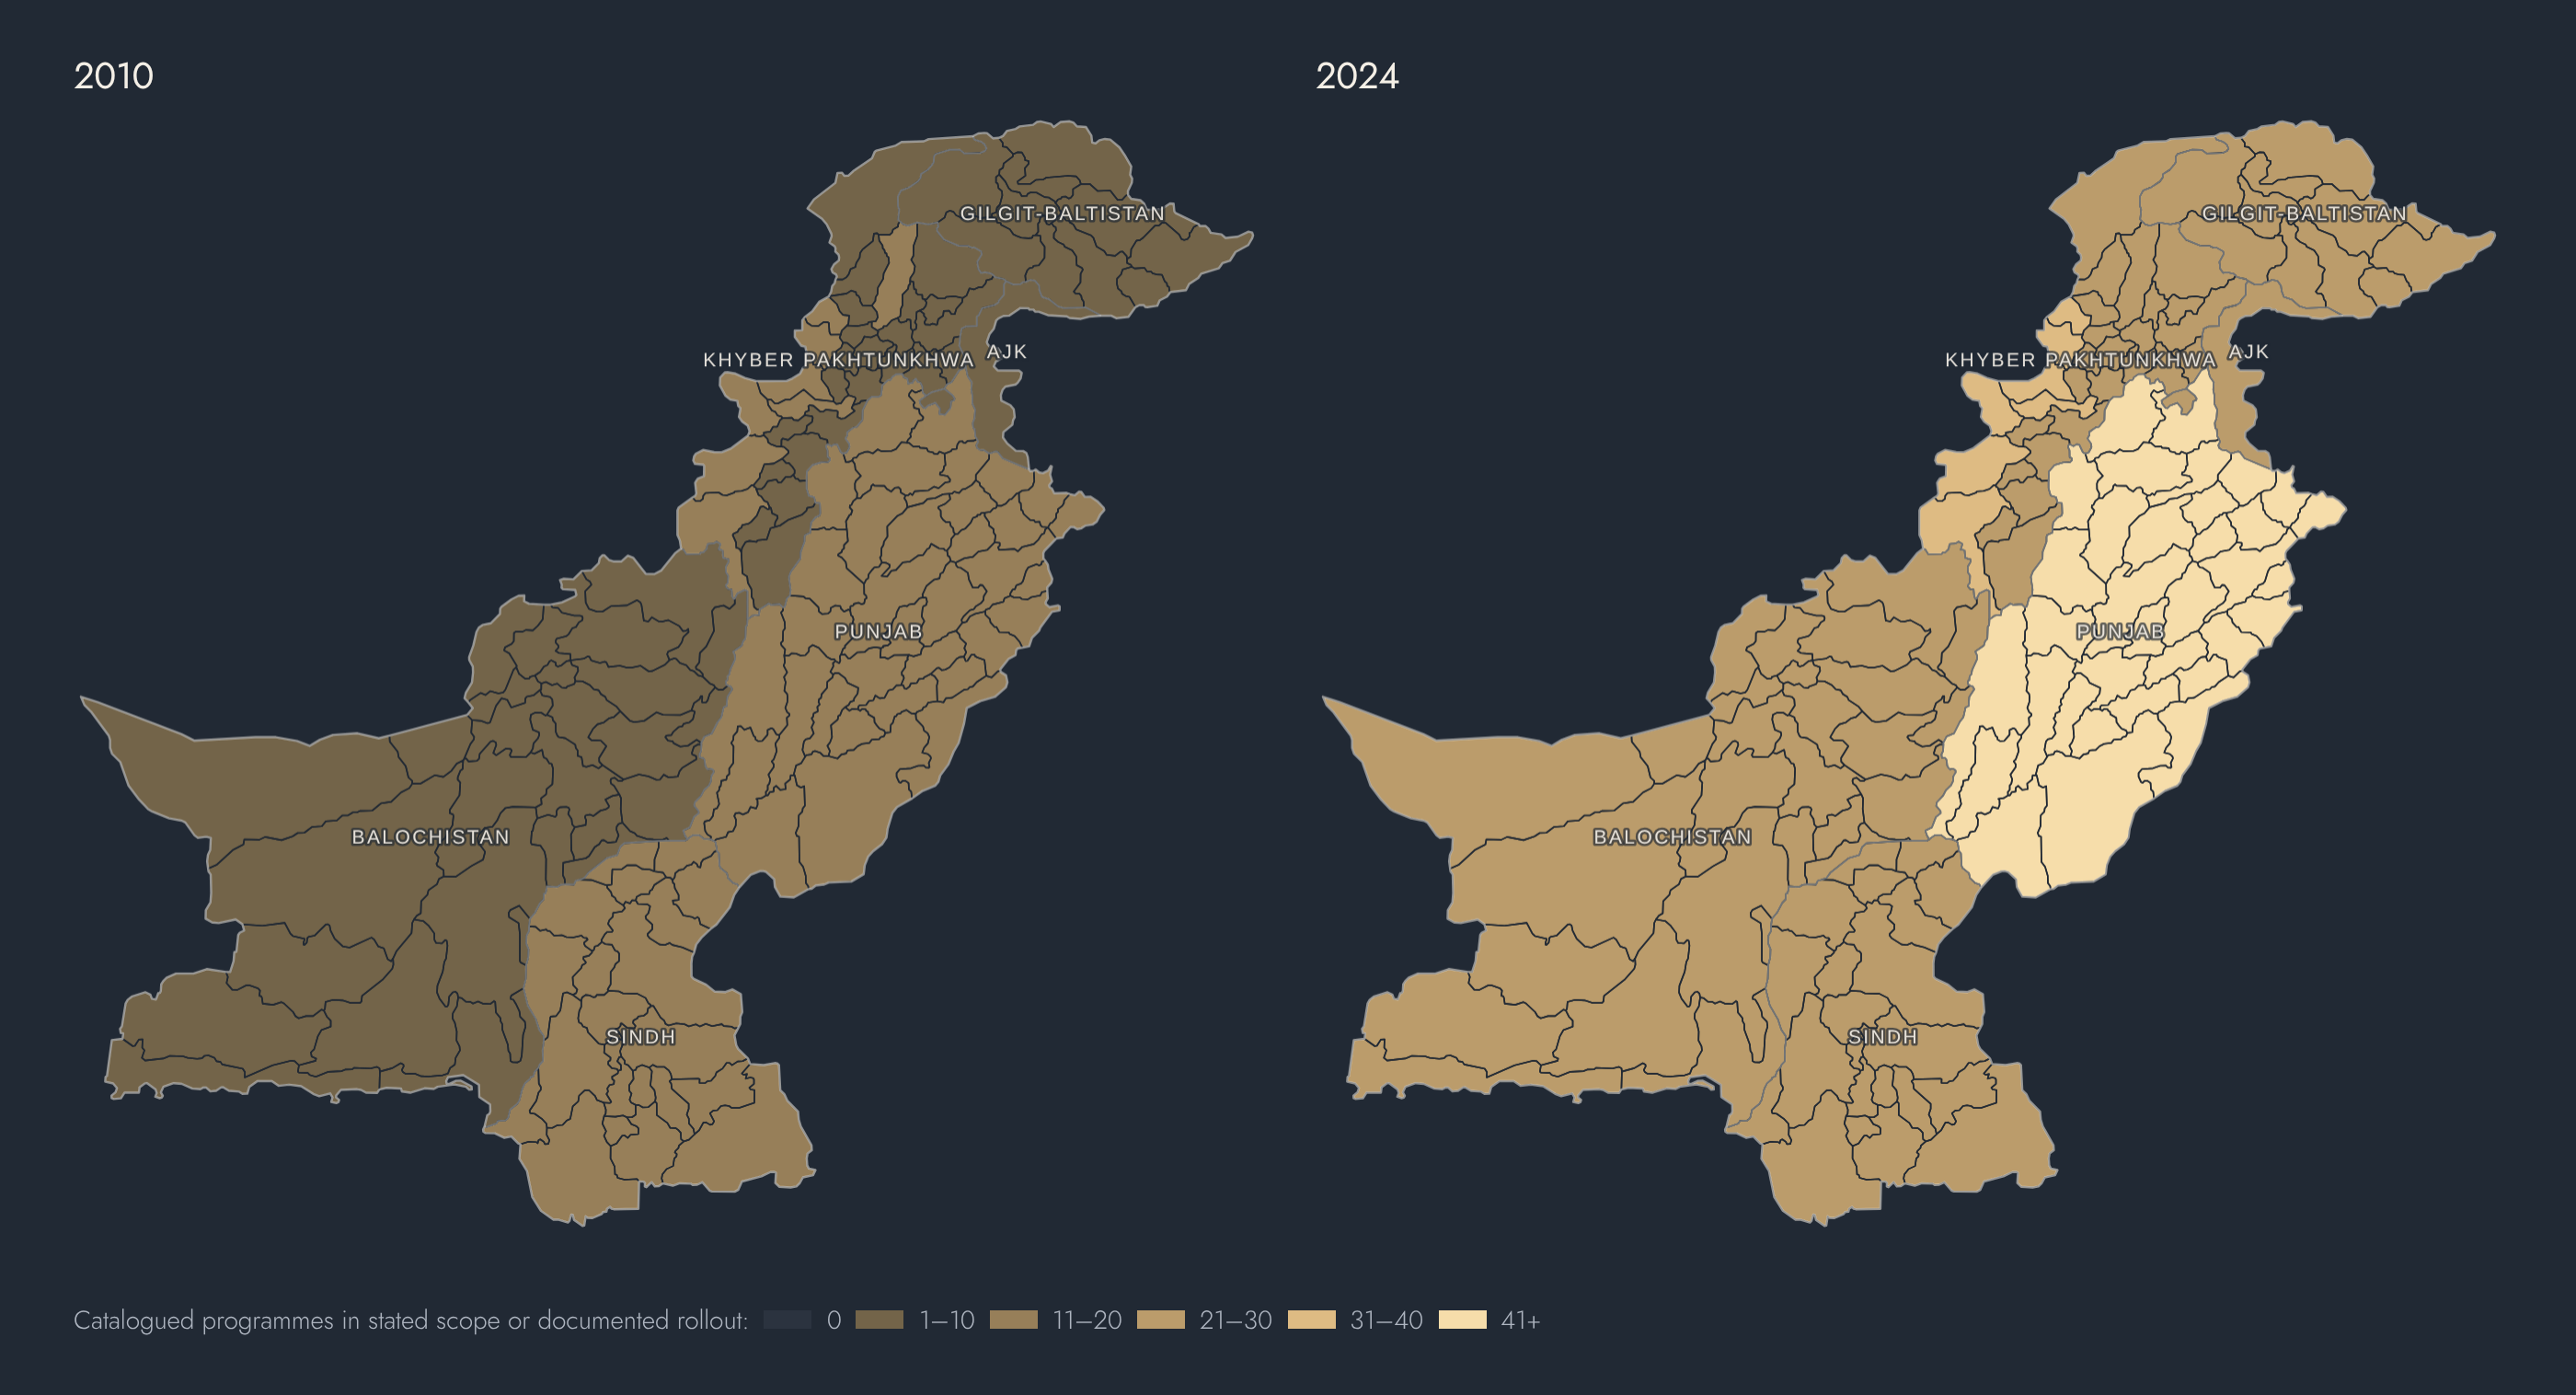
\includegraphics[width=\linewidth]{fig-density.png}
\caption{Catalogued programmes whose stated scope or documented rollout includes each district, 2010 and 2024. Scope is not treatment: national programmes count everywhere from their start year. Natural experiments are not counted.}
\end{figure}

\section{Documented footprints}
Rollout districts are shown on the map only where a named source lists them. Table~\ref{tab:fp} lists the 13 entries with such lists. ``Rest of scope'' means a source dates completion of the remaining districts only approximately; ``partial'' means later phases exist but are not dated here.

\begin{table}[ht]\centering\scriptsize
\caption{Entries with documented rollout districts}\label{tab:fp}
\begin{tabularx}{\linewidth}{lllllX}\toprule
ID & Entry & Phase years & Units & Final state & First source\\\midrule
P07 & Zewar-e-Taleem & 2017 & 15 & Full list & Punjab Social Protection Authority --- Zewar-e-Taleem Program \\
P14 & KP Sehat Card Plus & 2015 & 4 & Rest of scope by 2020 & Dawn --- Khattak launches health insurance scheme (16 Dec 2015) \\
P15 & Punjab health card & 2021, 2022 & 8 & Rest of scope by 2022 & Sehat Card Plus KP --- Programme history \\
P16 & Contracting out health units & 2003, 2007 & 2 & Partial & Public Health (2019) --- PPP in health service delivery in Sindh \\
P17 & PHFMC outsourcing & 2015 & 4 & Partial & Dawn --- Punjab to 'outsource' basic health project (14 May 2015) \\
P18 & Rescue 1122 & 2004 & 1 & Rest of scope by 2015 & Punjab Emergency Service --- Emergency Ambulance Service \\
P24 & PEF Education Vouchers & 2015 & 16 & Partial & The News --- PEF expands voucher scheme for students (22 Oct 2015) \\
P33 & Punjab Skills Development Fund & 2011 & 4 & Rest of scope by 2016 & PSDF Newsletter 2012, Vol. I \\
P40 & Punjab Safe Cities & 2016, 2019 & 8 & Full list & ARY News --- Punjab CM inaugurates Lahore Safe City project \\
P42 & FATA--KP merger & 2018 & 7 & Full list & Constitution (Twenty-fifth Amendment) Act, 2018 \\
P43 & New district creation & 2005, 2009, 2022, 2023 & 7 & Full list &  \\
P58 & Military operations & 2009, 2014 & 4 & Full list & ISPR announcements, compiled in BFRS / GTD event data \\
P64 & 2005 earthquake & 2005 & 6 & Full list & Earthquake Reconstruction \& Rehabilitation Authority --- affected districts \\
\bottomrule\end{tabularx}
\end{table}

\begin{figure}[ht]\centering
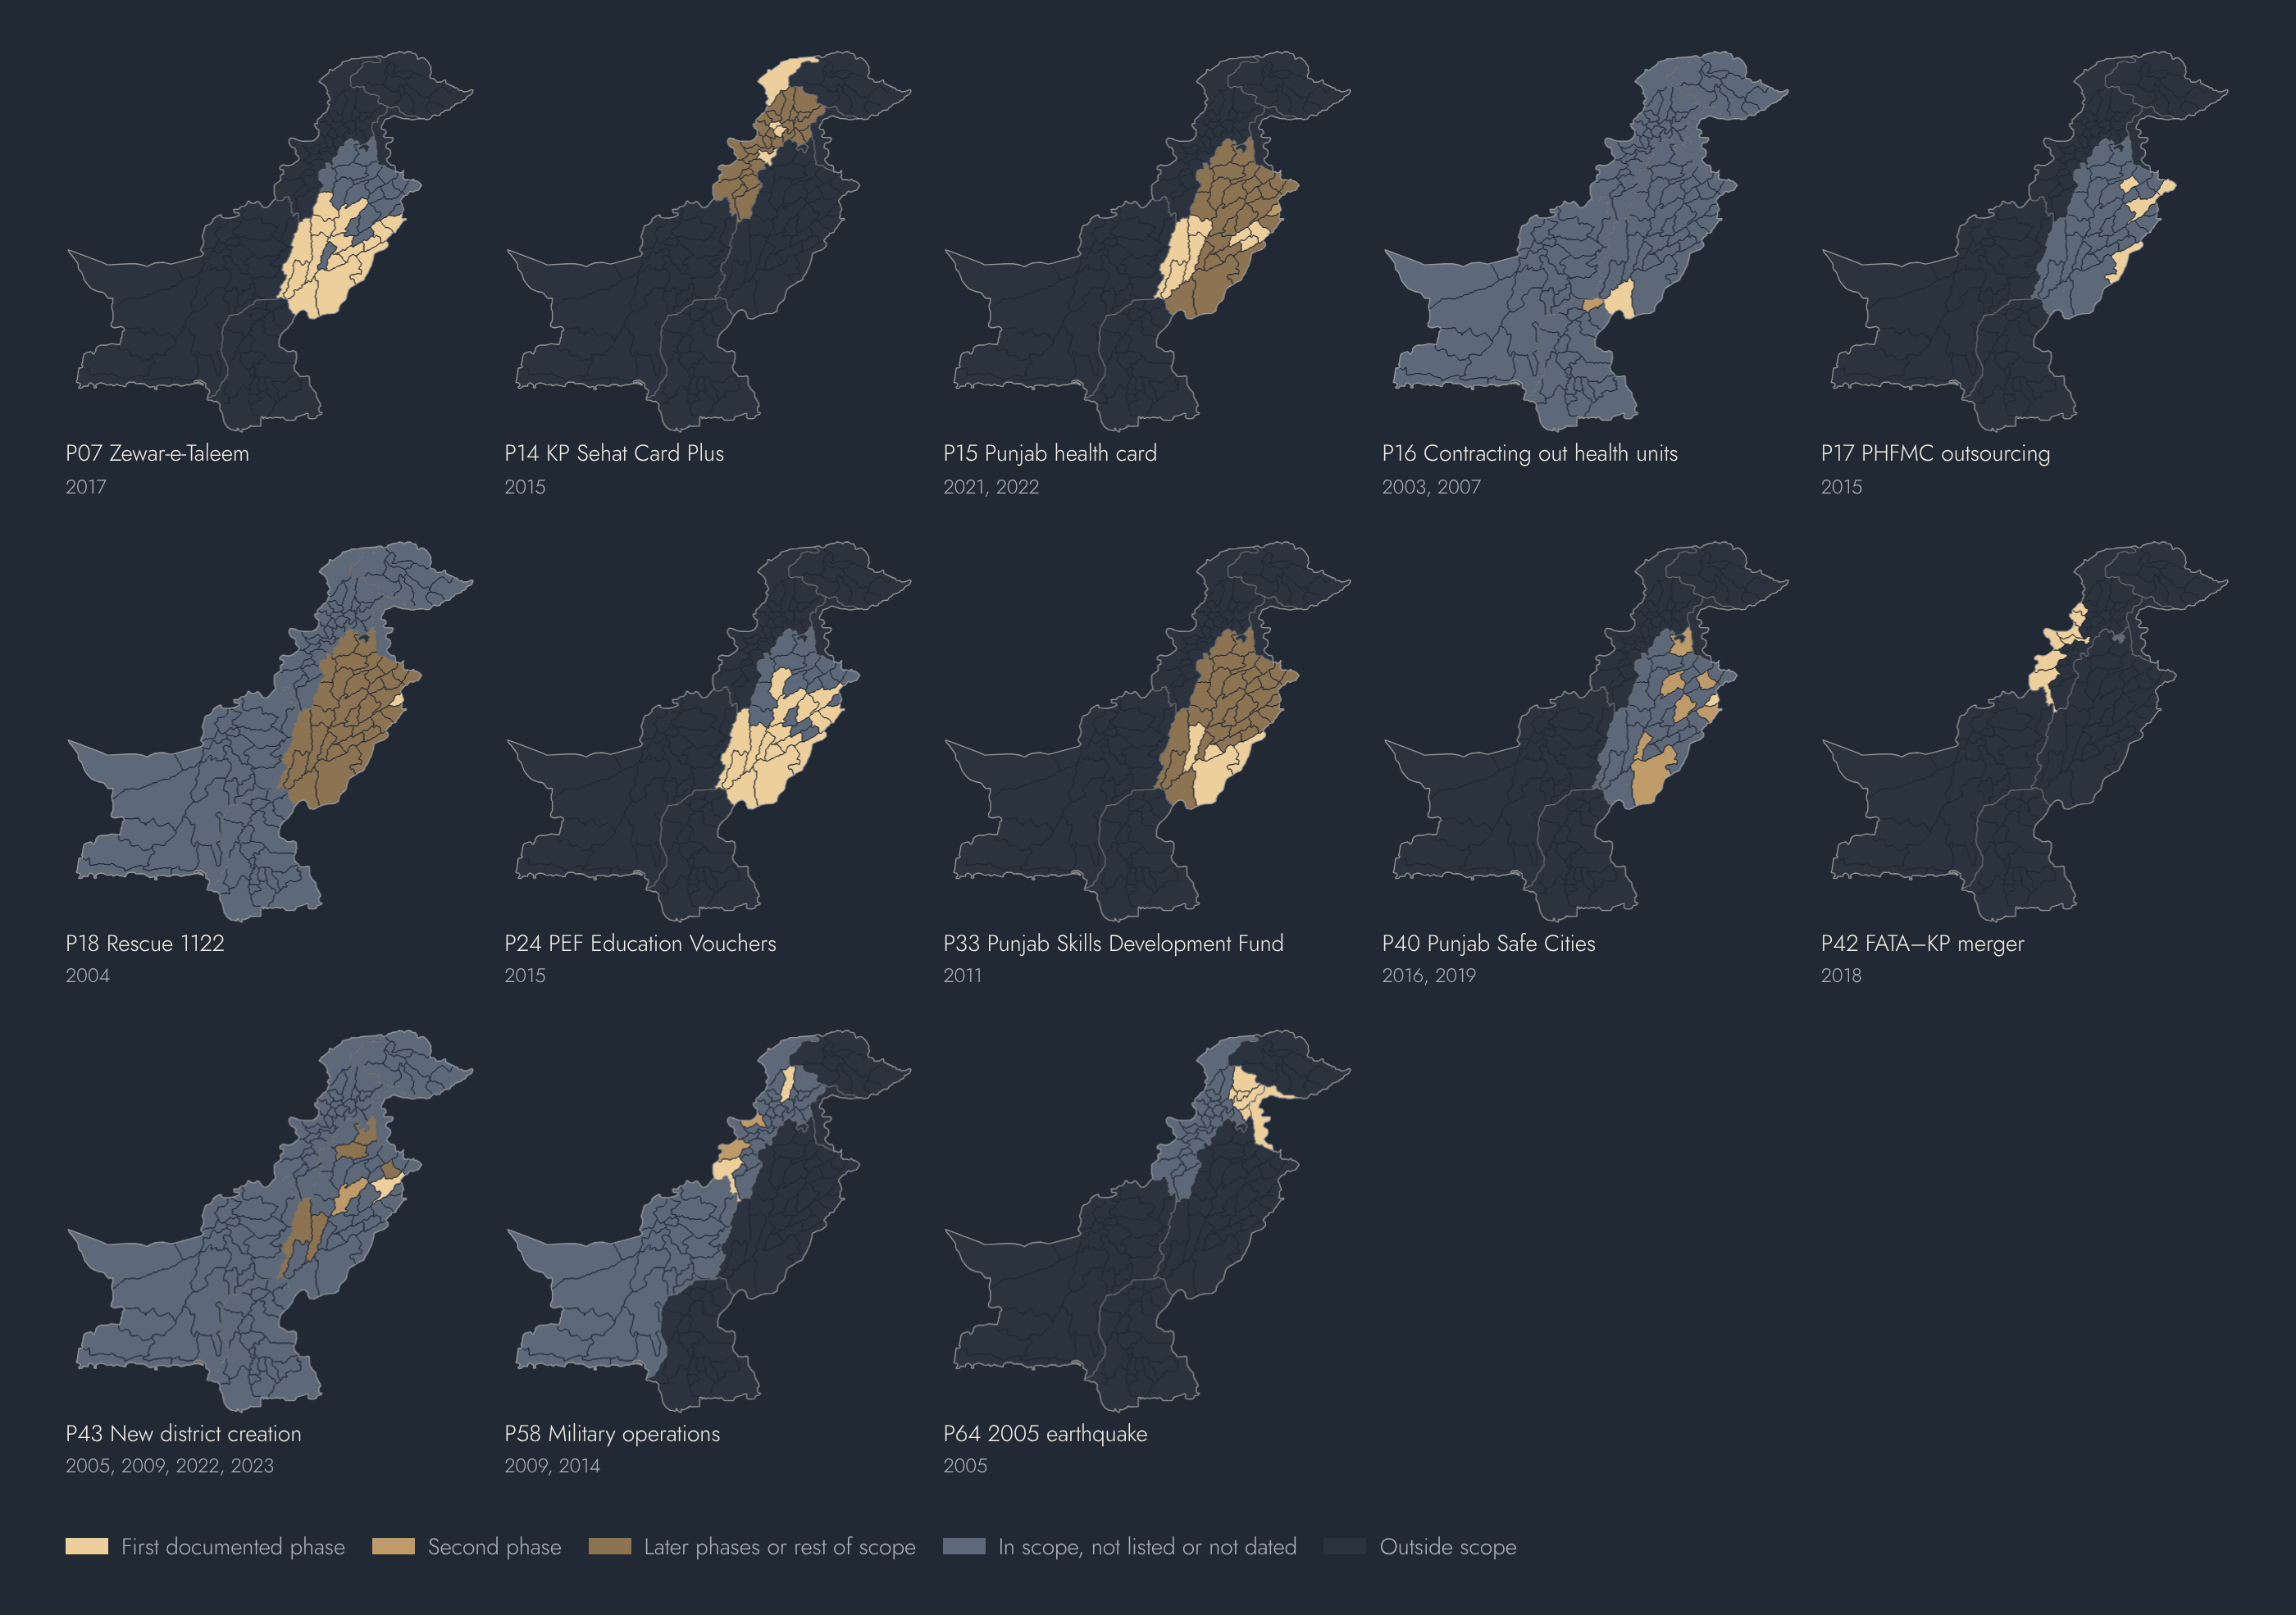
\includegraphics[width=\linewidth]{fig-footprints.png}
\caption{Documented footprints on 2019 boundaries.}
\end{figure}

\section{Corrections in this version}
Verifying footprints against primary sources changed three records from version 1.0:
\begin{itemize}
\item \textbf{P14 KP Sehat Card Plus.} v2.0: pilot districts named. Source: Dawn, 16 December 2015.
\item \textbf{P33 Punjab Skills Development Fund.} v2.0 correction: v1.0 listed Rahim Yar Khan instead of Muzaffargarh and dated the start to 2010. Source: PSDF Newsletter 2012, Vol. I.
\item \textbf{P40 Punjab Safe Cities.} v2.0 correction: v1.0 omitted Kasur. Source: Punjab Police press release, 2 January 2019.
\end{itemize}

\section{Limitations}
\begin{itemize}
\item Secondary sources disagree on dates routinely. Every date should be checked against the primary source named on the programme page before use.
\item Expected directions in the outcome matrix are hypotheses from mechanisms, not findings.
\item Evidence status was assigned by reading the literature cited; it will miss recent and unpublished work.
\item Several bibliography entries could not be verified from this build environment and are marked as such, with search links in place of DOIs.
\item Replication status of published studies has not been assessed.
\end{itemize}

\section{Access and citation}
All files are at \url{https://itssaqib.github.io/pakistan-evidence-catalogue/toolkit/} in CSV, JSON and Stata formats, with a Stata starter kit that includes the crosswalk, heterogeneity-robust estimators and a power calculation (Burlig, Preonas and Woerman 2020). Corrections are invited through the repository's issue forms.

\medskip\noindent Hussain, S. (2026). \emph{Pakistan Evidence Catalogue: staggered district-level programmes for causal impact evaluation}, version 2.0.0. \url{https://itssaqib.github.io/pakistan-evidence-catalogue/}

\end{document}
